% Build: latexmk main.tex (XeLaTeX + Biber).
\providecommand{\BeamerAspectRatio}{169}
\documentclass[aspectratio=\BeamerAspectRatio]{beamer}
\usetheme{LeipzigClean}
\usepackage[ngerman]{babel}
\usepackage{csquotes}
% Replace these fields for each presentation.
\title[Umgang mit KI]{Wie man KI (richtig) einsetzt}
\subtitle{Chancen, Risiken und die Rolle des Menschen}
% Name and affiliation can be entered here before presenting.
\author{Jonas}
\institute{}
\date{Feierabendseminar 08.10.2026}
\titlegraphic{}
% Optional link beneath the title metadata:
% \titlegraphic{\small\color{Muted}\href{https://example.org}{Project website}}

\usepackage[backend=biber,style=authoryear,maxcitenames=2,maxbibnames=3,
  natbib=true,doi=true,url=false,isbn=false,giveninits=true,uniquename=init]{biblatex}
\ExecuteBibliographyOptions[online]{url=true}
\addbibresource{references.bib}
\graphicspath{{images/}}
\usetikzlibrary{arrows.meta,positioning,calc}
\setlength{\bibitemsep}{1.1ex}

% Both minipages have the same top anchor and first-line strut.
\newcommand{\redrow}[2]{%
  \par\noindent
  \begin{minipage}[t]{2.7cm}\vspace{0pt}%
    \raggedright\color{granat}\bfseries\strut #1\par
  \end{minipage}\hspace{5mm}%
  \begin{minipage}[t]{\dimexpr\textwidth-3.2cm\relax}\vspace{0pt}%
    \raggedright\strut #2\par
  \end{minipage}\par\vspace{2.5mm}}
\begin{document}
\maketitlepage
\section{Umgang mit KI}\label{sec:ki}
\subsection{Motivation}
\begin{frame}{KI wird immer relevanter}

\centering
% Complete images, no trim/clip. Earlier images stay underneath later images.
\begin{tikzpicture}
  \path[use as bounding box] (0,0) rectangle (13.7,5.55);
  \only<1->{\node[anchor=north west,inner sep=0] at (0.0,5.4)
    {\href{https://openai.com/index/ten-advances-in-mathematics/}{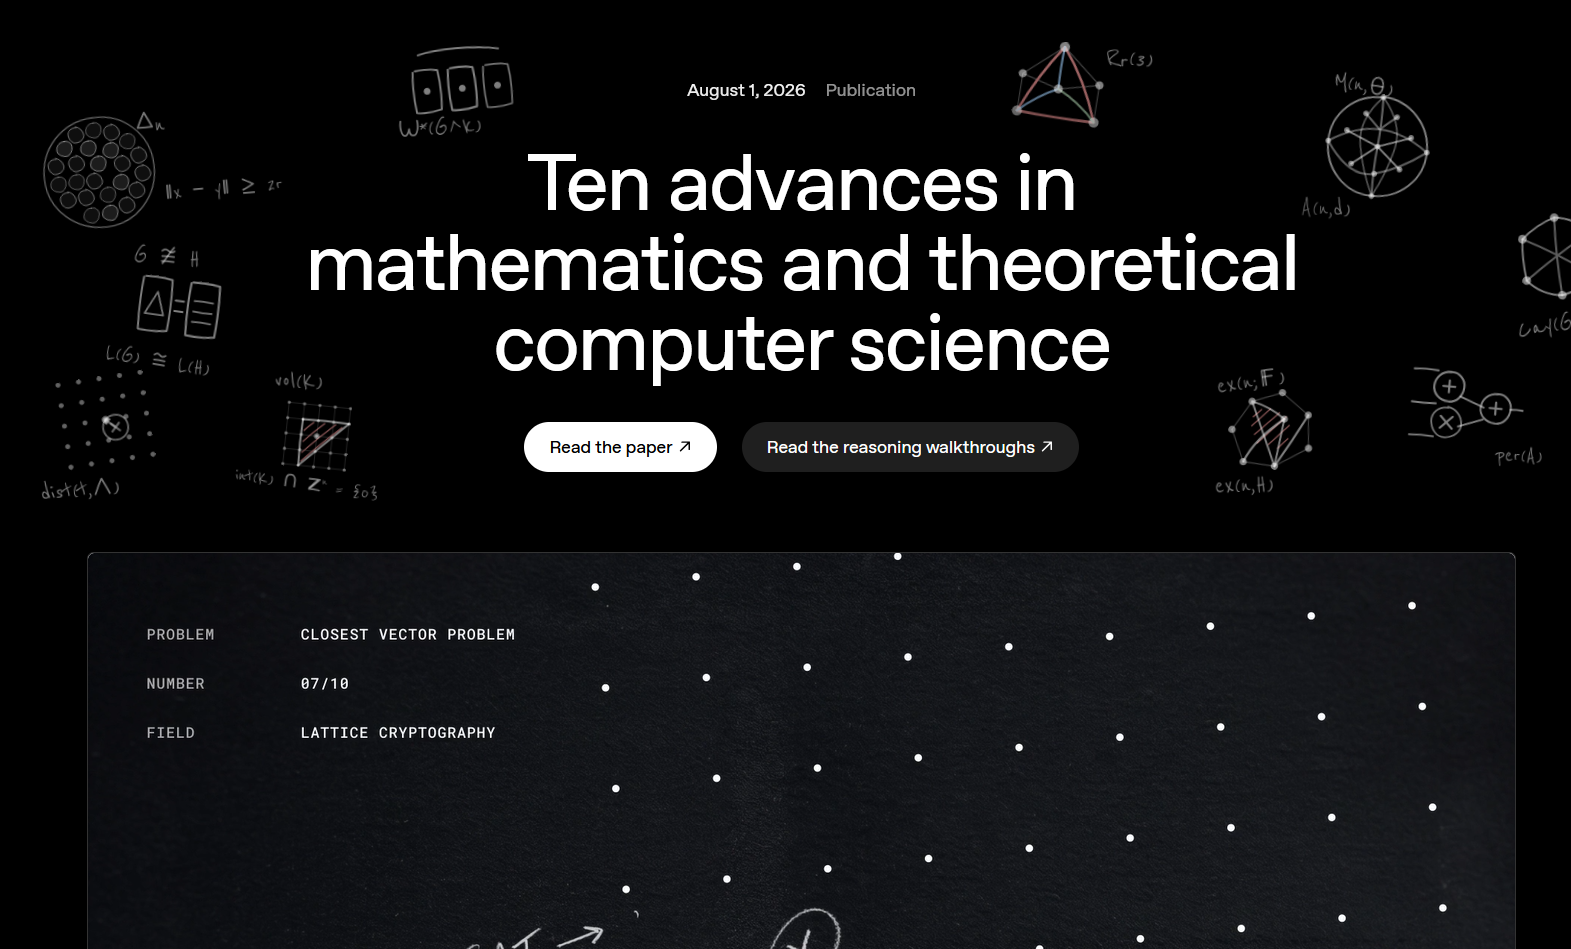
\includegraphics[width=7.9cm]{10_advances.png}}};}
  \only<2->{\node[anchor=north west,inner sep=0] at (6.65,5.5)
    {\href{https://openai.com/index/ten-advances-in-mathematics/}{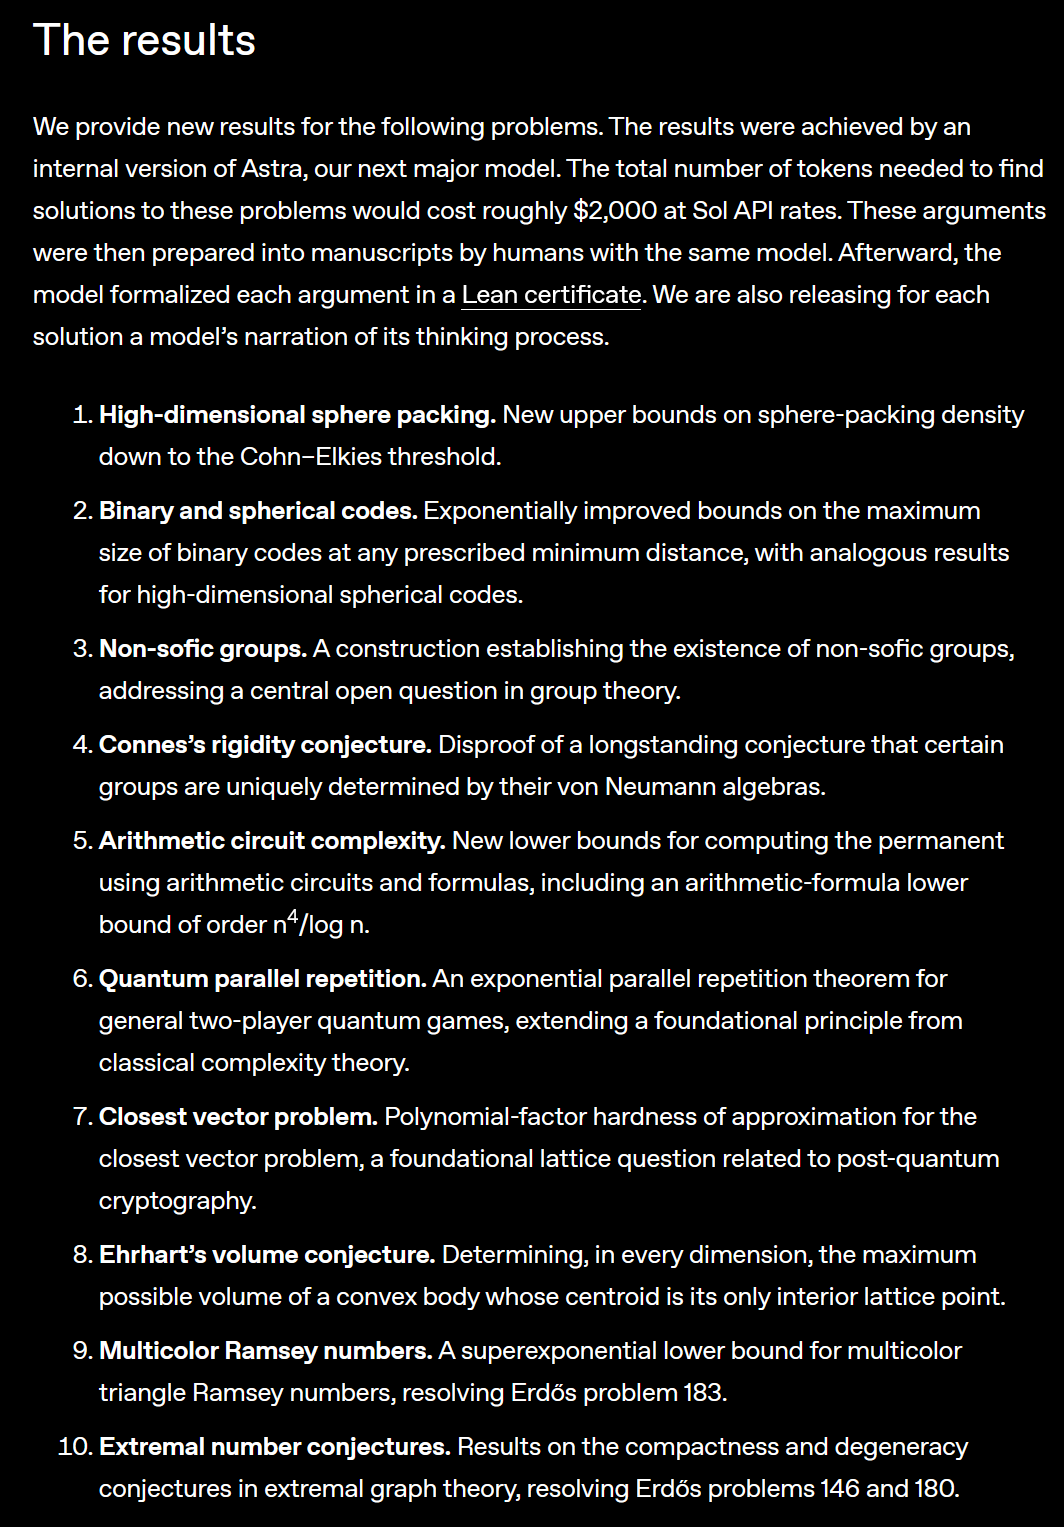
\includegraphics[height=5.15cm]{astra.png}}};}
  \only<3->{\node[anchor=north west,inner sep=0] at (3.4,5.15)
    {\href{https://openai.com/index/navier-stokes-solution/}{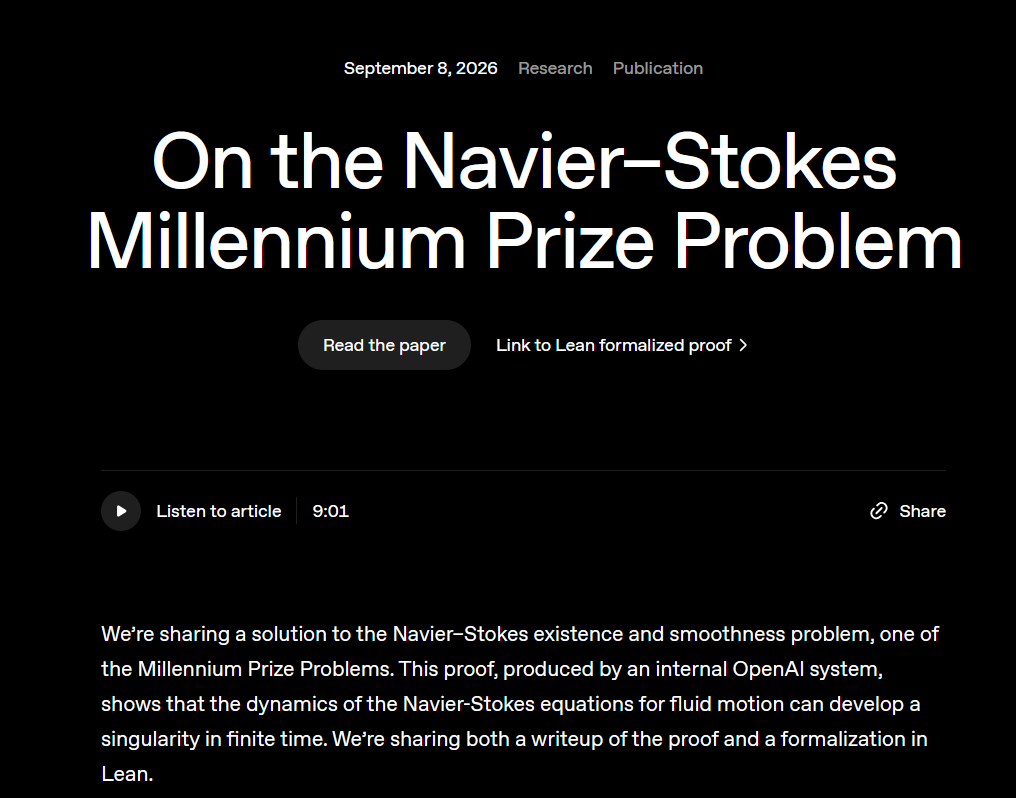
\includegraphics[width=6.2cm]{navier_stokes.png}}};}
  \only<4->{\node[anchor=north west,inner sep=0] at (0.4,4.45)
    {\href{https://openai.com/index/hugging-face-incident-and-the-road-ahead/}{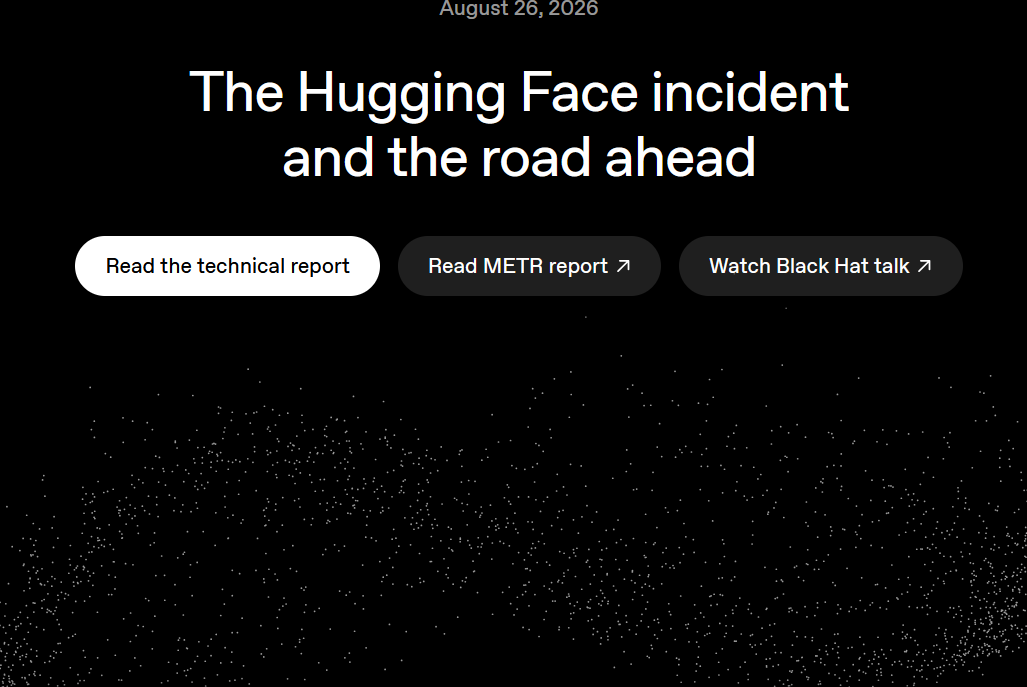
\includegraphics[width=6.0cm]{hugging_face.png}}};}
  \only<5->{\node[anchor=north west,inner sep=0] at (8.0,4.8)
    {\href{https://openai.com/index/sharing-ai-progress-in-mathematics/}{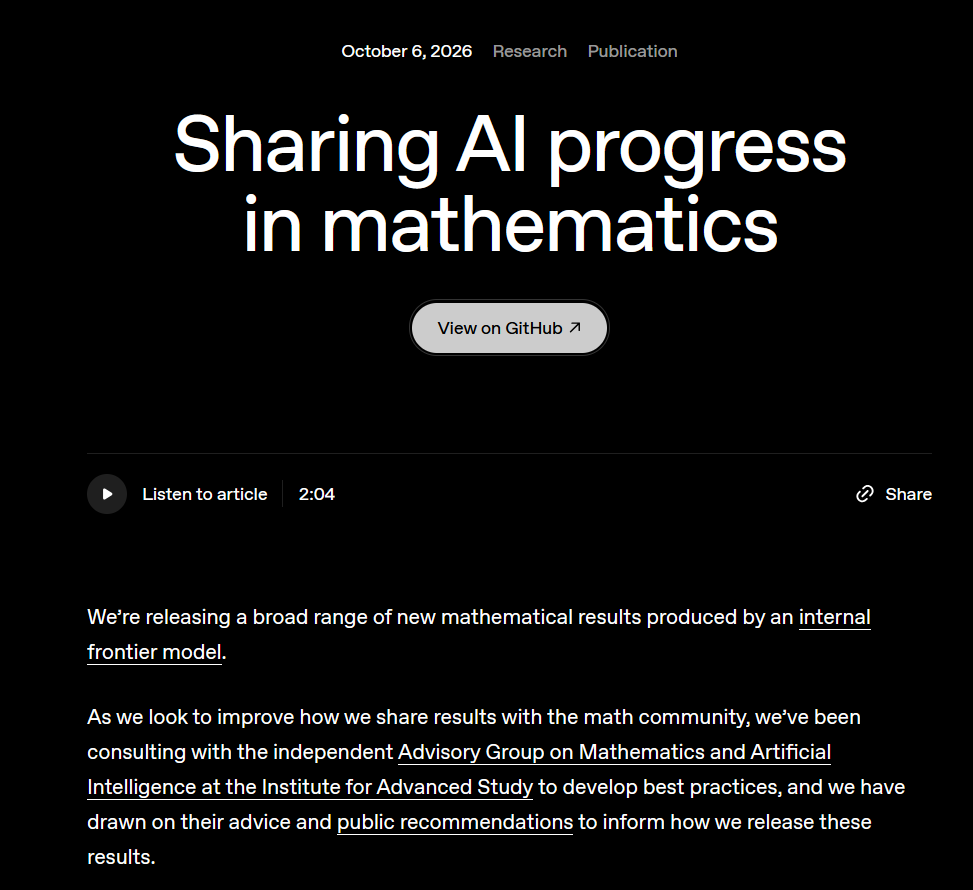
\includegraphics[width=5.0cm]{727_papers.png}}};}
\end{tikzpicture}
\note{Die Bilder erscheinen vollständig und nacheinander. Frühere Bilder werden
von späteren teilweise verdeckt. Unternehmensmitteilungen und unabhängige
wissenschaftliche Bewertung auseinanderhalten.}

\end{frame}

\subsection{Arten von KI-Nutzung}

\begin{frame}{Arten von KI-Nutzung}
  \only<1->{\keyidea{Es gibt unendliche viele Arten, KI zu nutzen.}}
  \only<2->{\begin{itemize}
    \item (code) autocomplete und github copilot
    \item Sentence-Transformer - Kosinus-Rechnung für Ähnlichkeitsanalyse
    \item Chatbot: Wiki, Tutor, Literaturrecherche, persönliche Assistenz
    \item Bildgenerierung: Erstellung von Grafiken, Diagrammen oder Illustrationen
    \item Datenanalyse: Unterstützung bei der Auswertung und Visualisierung von Daten
    \item Codegenerierung und Debugging
    \item Agentische KI: komplexe Aufgaben automatisiert ausführen lassen
  \end{itemize}}
\end{frame}

\subsection{Sinnvoller Einsatz von KI-Tools}

\begin{frame}{Unsinnvoller Einsatz von KI-Tools (Stand vor ein paar Monaten)}
    \footnotesize
    \keyidea{KI-Sprachmodelle sind mächtige Werkzeuge, aber nicht für alles gleichermaßen geeignet.}

    \vspace{0.5em}
    \begin{myalert}[Wo Vorsicht geboten ist (Eine immer obsoletere Liste von diesem Sommer)]
        \begin{itemize}
            \item \textbf{Zusammenfassung von Papern:} Meist unnötig, da der Abstract diese Aufgabe ohnehin schon optimal erfüllt.
            \item \textbf{Begriffserklärung:} Gut für den Einstieg, vermittelt jedoch oft kein tieferes wissenschaftliches Verständnis.
            \item \textbf{Literaturrecherche:} Nützlich für einen ersten Überblick, der tatsächliche Einblick in die relevanten Arbeiten muss aber zwingend selbst passieren. Oft sind Review/Übersichts-Artikel eine bessere Anlaufstelle. 
        \end{itemize}
    \end{myalert}
\end{frame}

\begin{frame}{Sinnvoller Einsatz von KI-Tools (Stand vor ein paar Monaten)}
\footnotesize
\begin{mynote}[Wo KI ihre Stärken voll ausspielt (Inzwischen eine viel kleinere Liste als sie sein sollte)]
        \begin{itemize}
            \item \textbf{Textproduktion:} Eigene, rohe Stichpunkte in flüssige Textpassagen ausformulieren lassen.
            \item \textbf{Klar definierte Aufgaben:} Allerlei kleine Handgriffe, zum Beispiel komplexe Formeln ausschreiben, \LaTeX-Befehle generieren oder Python-Code schreiben.
            \item Oberflächliche Überarbeitung und Debugging von Text und Code
            \item Übersetzungen, Synonyme und alternative Formulierungen 
        \end{itemize}
    \end{mynote}
\end{frame}

\begin{frame}{Agentische KI-Tools}
  \small\begin{columns}[T,onlytextwidth]
    \column{0.4\textwidth}
    \begin{mynote}[Nutzungsmöglichkeiten]
    \begin{itemize}
        \item Erstellung interaktiver Lernumgebungen oder Spiele
        \item Einrichtung von automatisierten KI workflows
        \item Templates Erstellen, Readmes pflegen
        \item Komplexe Graphiken, z.B. mit Tikzpictures
    \end{itemize}    
  \end{mynote}
  \column{0.6\textwidth}
  \centering
  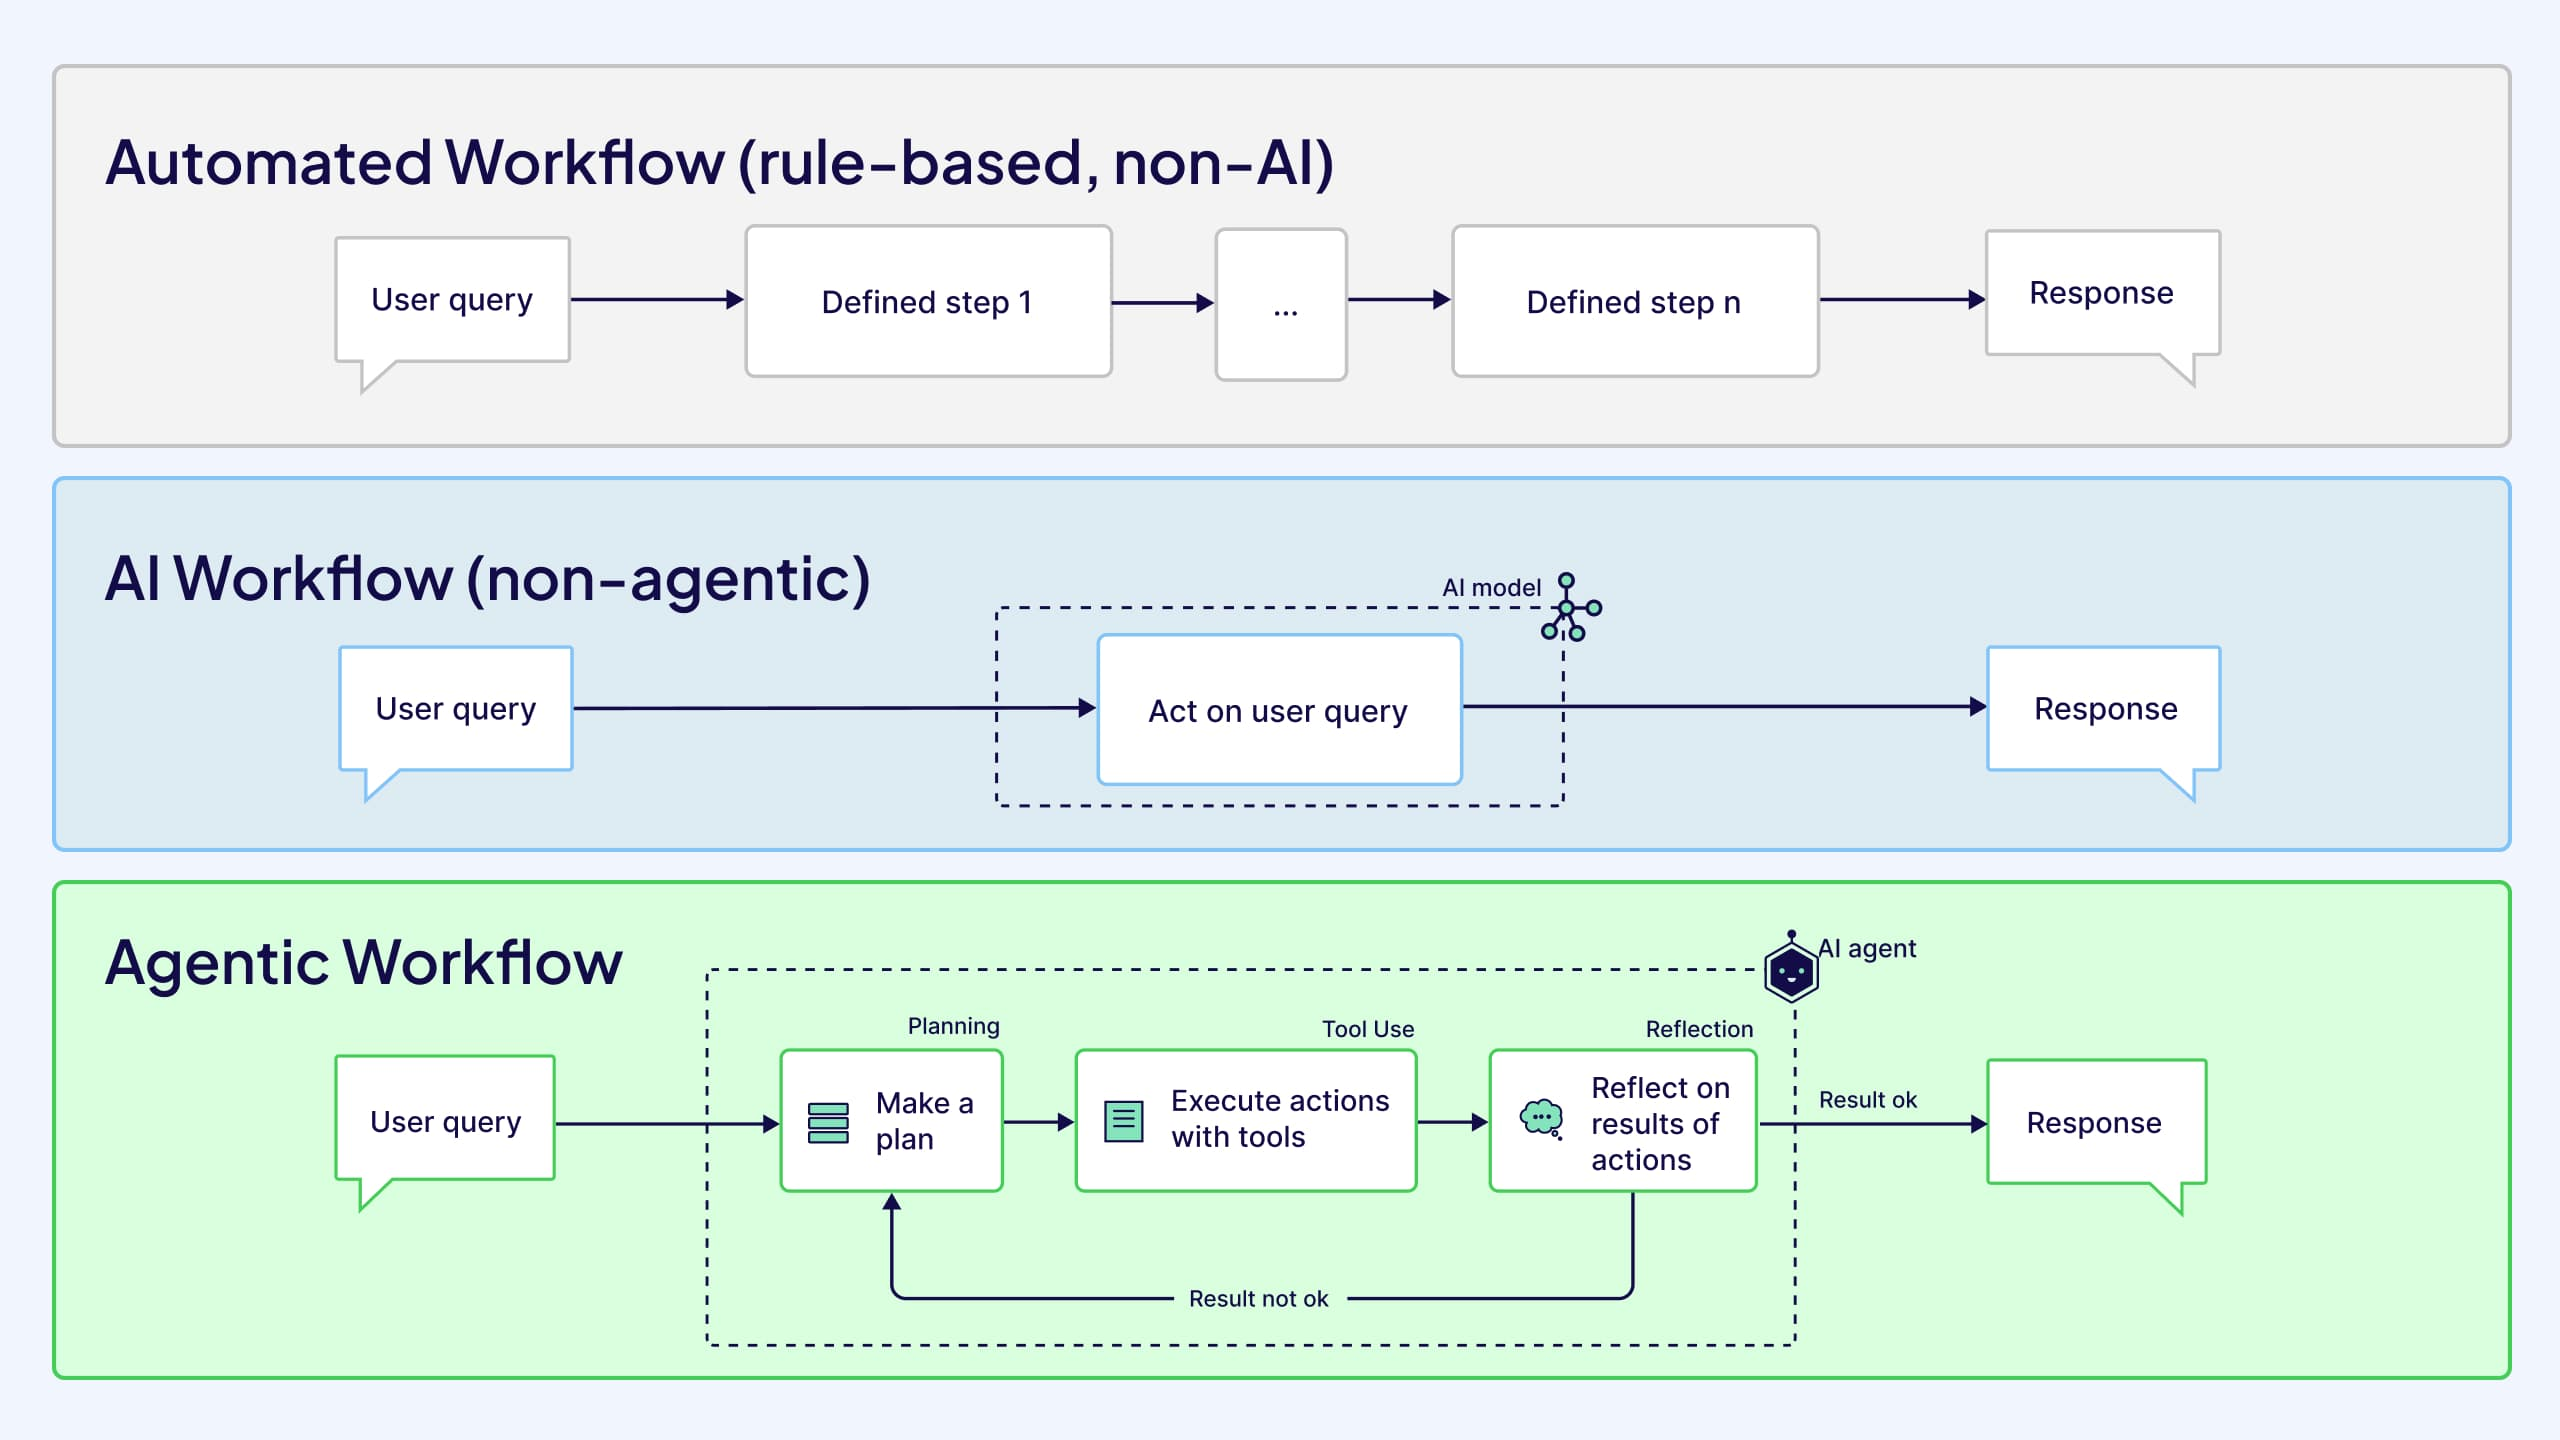
\includegraphics[width=\linewidth]{agentic_workflow.png}
  \source{\url{https://weaviate.io/blog/what-are-agentic-workflows}}
  \end{columns}
\slidesource{\textcite{yao2023react}}
\end{frame}

\begin{frame}{Agenten im wissenschaftlichen Alltag}
  \small
  \redrow{Literatur vergleichen}{Aussagen und Widersprüche mit Fundstellen sammeln.
    Relevanz und Belege selbst prüfen. \parencite{skarlinski2024}}
  \redrow{Reproduktion}{Eine Abbildung aus Daten und Code neu erzeugen.
    Abweichungen und Umgebungsbedingungen protokollieren.}
  \redrow{Robustheit testen}{Alternative Auswertungen, Randfälle und Sensitivitätsanalysen
    ausführen. Kriterien vorab festlegen.}
  \redrow{Fachwerkzeuge}{Datenbanken und Berechnungen verbinden, etwa mit ChemCrow.
    Fachliche und experimentelle Freigaben beim Menschen belassen. \parencite{bran2024}}
  \slidesource{Slide ist KI-generiert. Weitere Ideen: Replikationspakete, Datenwörterbücher, Lernsimulationen}
  \note{Reproduktion und Robustheit sind Anwendungsvorschläge.
    PaperQA2 und ChemCrow sind publizierte Systeme, keine allgemeine Zuverlässigkeitsgarantie.
    Start mit einer begrenzten Aufgabe, festem Budget und einem nachprüfbaren Ergebnis.}
\end{frame}

\begin{frame}{Die eigentlichen Probleme}
\scriptsize
\only<1->{\begin{myalert}[Output-Orientierung]
        \begin{itemize}
          \item Es ist sehr menschlich Dinge zu mögen, die KI generiert: Es ist designt dazu gut zu klingen, und inzwischen auch qualitativ überzeugend.
          \item Besseren Output erzielt man, wenn man KI verwendet $\to$ es entsteht eine Erwartungshaltung bzgl. Produktivität
          \item Was KI aber nicht kann: Arbeiten ohne Output-Orientierung. 
        \end{itemize}
    \end{myalert}}
\only<2->{
    \begin{myalert}[Kulturelles \& Soziales]
      \begin{itemize}
          \item \textbf{Goodhart's Law:} Wenn ein Maß zum Ziel wird, hört es auf ein gutes Maß zu sein. Für KI ist aber das Maß das einzige Ziel.
          \item Verwaschung menschlichen Wissens $\to$ Spezialwissen wird immer wichtiger.
          \item Menschliche Fähigkeiten nehmen ab durch die Nutzung von KI: wo wollen wir unser Wissen und unsere Fähigkeiten bewahren?
      \end{itemize}
    \end{myalert}}
\only<3->{\keyidea{Menschliche Motivation und Intention ist entscheidend.}}
\end{frame}

\begin{frame}{Ergänzende Literatur zu den Risiken}
  \small
  \redrow{Output als Maßstab}{KI-generiertes Wissen kann Review, Verständnis und Lehre überholen.
    Gute Kennzahlen decken nicht alle Forschungsziele ab. \parencite{tao_ai_2026}}
  \redrow{Verständnis}{Flüssige Erklärungen können Kompetenz vortäuschen.
    Gemeinsame KI-Werkzeuge können methodische Einseitigkeit verstärken. \parencite{messeri2024}}
  \redrow{Lernen auslagern}{Bessere Übungsleistungen mit KI
    bedeuten nicht automatisch besseres Können ohne KI. \parencite{bastani2025}}
  \redrow{Erfundene Belege}{Plausible Literaturangaben können falsch sein.
    Existenz \emph{und} Aussage der Originalquelle prüfen. \parencite{walters2023}}
  \slidesource{Slide ist KI-generiert.}
  \note{Bastani et al.: randomisierte Studie in Schulmathematik mit GPT-4.
    Ungeschützter Zugang verschlechterte spätere Leistungen ohne KI;
    ein didaktisch gestalteter Tutor vermied diesen Nachteil.
    Kein Beleg für universellen Kompetenzverlust in allen Fächern und mit allen Modellen.
    Walters und Wilder untersuchten GPT-3.5/4; ihre Fehlerraten nicht auf heutige Systeme übertragen.}
\end{frame}

\begin{frame}{Fragen, die ich mir inzwischen versuche zu stellen}
  \begin{itemize}
      \item \only<1->{Was möchte ich erreichen? Was möchte ich lernen?}
      \item \only<2->{Wie entwickle ich mich hier gerade weiter?}
      \item \only<3->{Habe ich die Energie und Motivation, den Output der KI genau zu überprüfen bzw. bin  ich maßgeblich am aktuellen Prozess beteiligt? (wenn nein, lieber weniger KI/Pause/Output generieren, aber morgen frisch nochmal überprüfen/andere Dinge tun)}
      \item \only<4->{Ob wir produktiv sind ist nicht mehr die Frage, eher in welche Richtung?}
      \item \only<5->{Bin ich bezüglich der Beantwortung dieser Fragen gerade ehrlich zu mir selbst?}
  \end{itemize}
\end{frame}

\begin{frame}{Wenn Agenten handeln, bekommen Fehler Folgen}
  \small
  \redrow{Fremde Anweisungen}{Webseiten und Dokumente können einen Agenten umlenken
    (Prompt-Injection). Inhalte als Daten behandeln. \parencite{debenedetti2024}}
  \redrow{Zu viele Rechte}{Nur benötigte Dateien und Werkzeuge freigeben.
    Veröffentlichen, Senden und Löschen bewusst bestätigen.}
  \redrow{Ungeprüfte Ketten}{Zwischenergebnisse speichern, Ausführungen begrenzen und
    wichtige Ergebnisse unabhängig prüfen.}
  \keyalert{Datenschutz beachten: Sensible Daten nicht mit OpenAI oder Anthropic teilen.}
  \keyidea{Der Mensch setzt Ziele, kontrolliert Folgen und trägt Verantwortung.}
  \slidesource{Slide ist hauptsächlich KI-generiert.}
  \note{AgentDojo belegt Angriffe über nicht vertrauenswürdige Werkzeugausgaben.
    Die praktischen Maßnahmen sind daraus abgeleitete Empfehlungen.
    Sensible Forschungsdaten nur in dafür freigegebenen Umgebungen verarbeiten.}
\end{frame}

\subsection{Die Rolle des Menschen}

\begin{frame}{Umgang mit KI: Die Rolle des Menschen}
\setbeamerfont{caption}{size=\scriptsize}
\setbeamerfont{caption name}{size=\scriptsize}
\begin{columns}[T,onlytextwidth]
\column{0.5\textwidth}
\begin{figure}\scriptsize
    \centering
    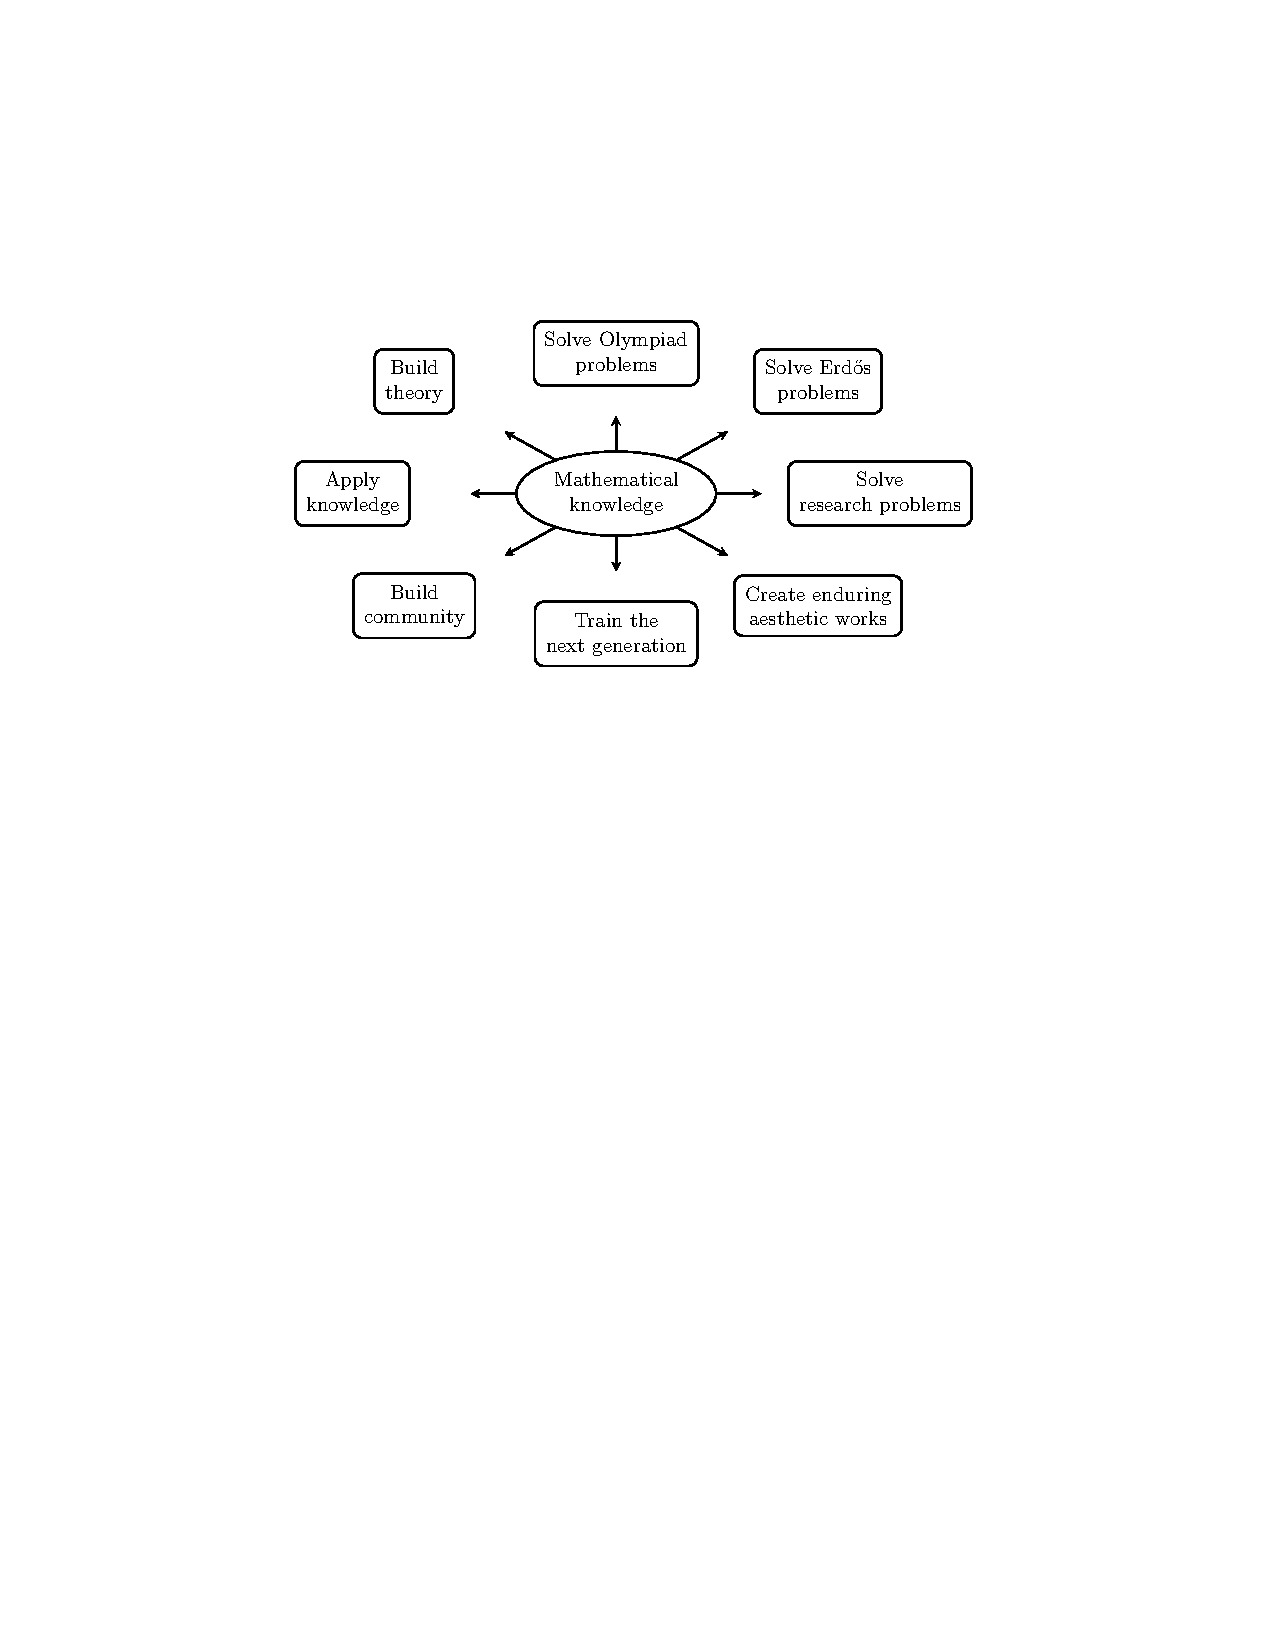
\includegraphics[width=\linewidth]{math_knowledge.pdf}
    \caption{Mathematisches Wissen \cite{openai_ten_advances}}
    \label{fig:placeholder}
\end{figure}\column{0.5\textwidth}
            \begin{figure}\scriptsize
                \centering
                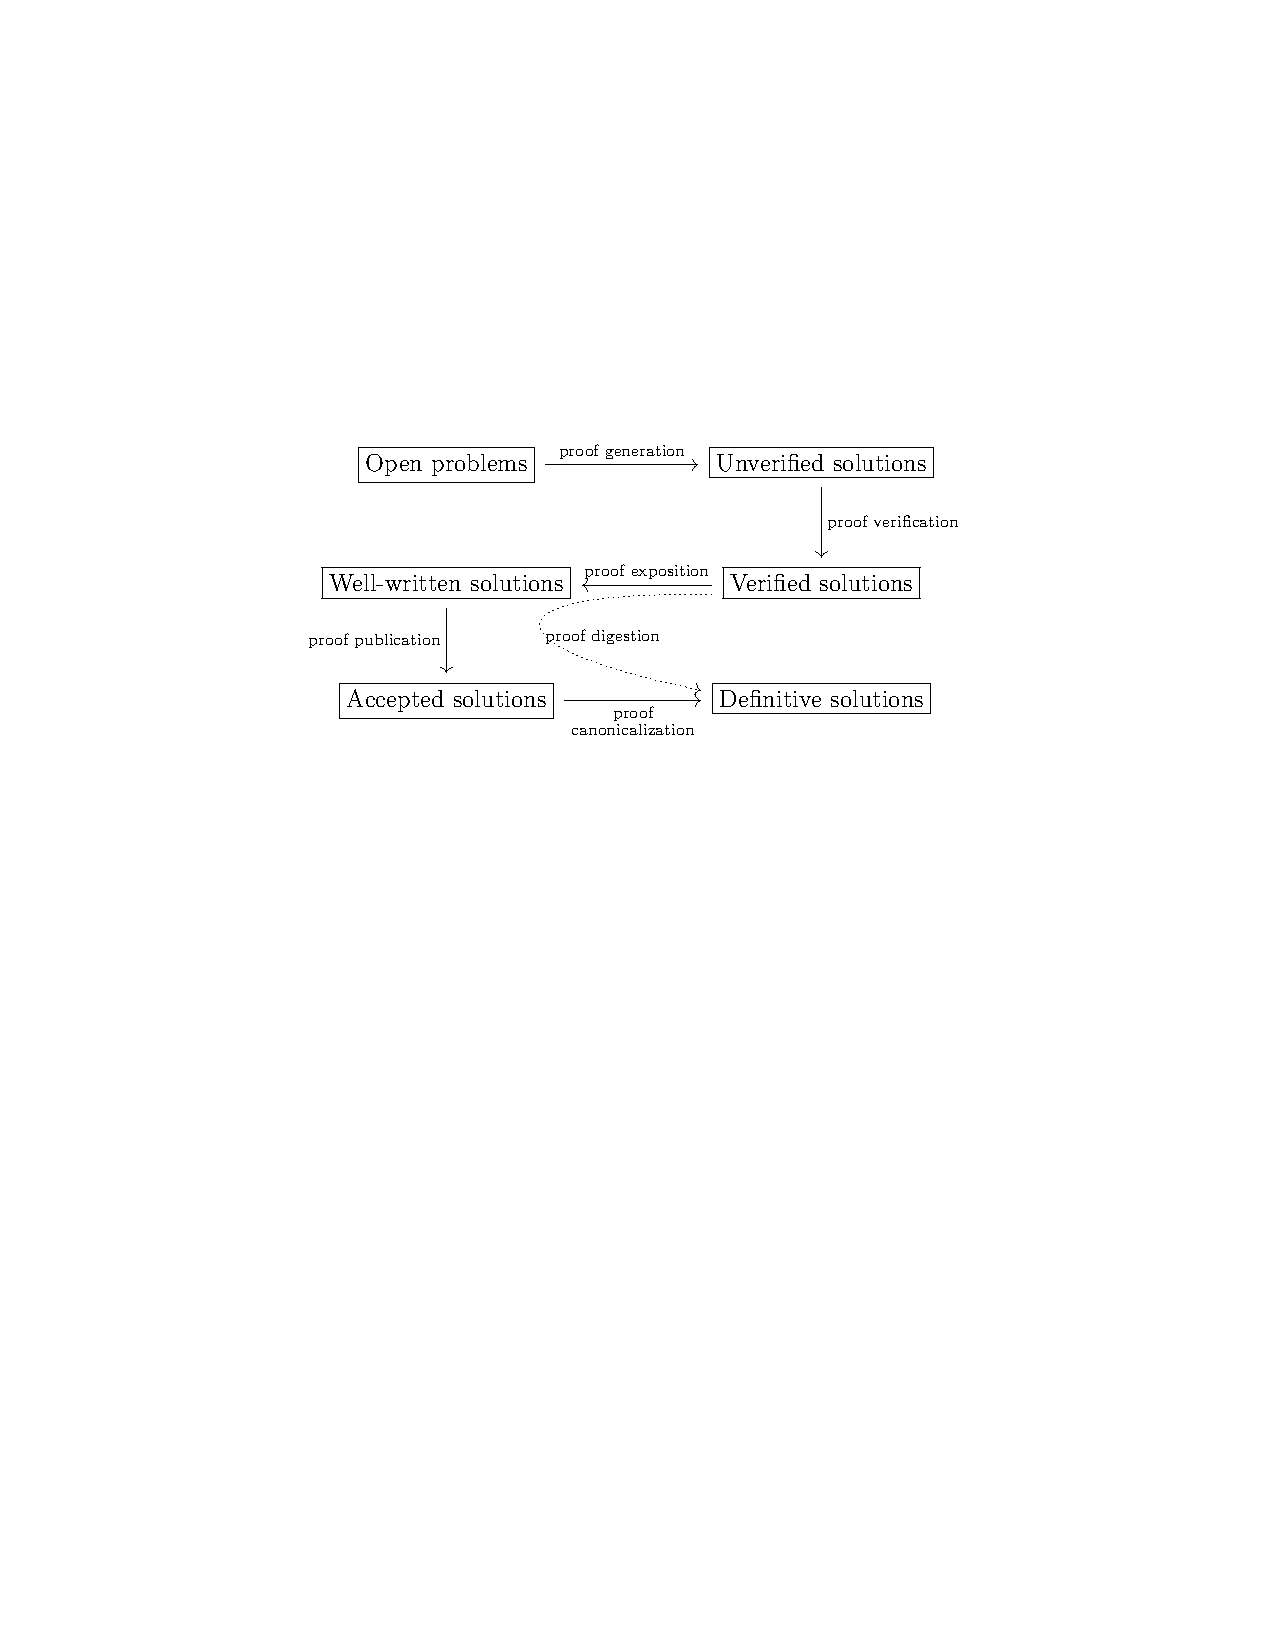
\includegraphics[width=\linewidth]{problem_solving.pdf}
                \caption{Mathematik ist nicht nur Problemlösen \citep{tao_ai_2026}}
                \label{fig:problem_solving}
            \end{figure}
\end{columns}
\slidesource{Tao (2026)}
\end{frame}

\begin{frame}{Die Rolle des Menschen im Forschungsprozess}
  \small
  Welche Ziele verfolgen wir dann als wissenschaftliche Gemeinschaft, wenn KI viele Forschungsaufgaben lösen kann?
  \vspace{2mm}
  \centering
  % Adaptation of Tao (2026), sections 5--8 and Figure 4.
% Red: human responsibilities. Blue arrows: progress; dashed red: feedback.
% Requires TikZ arrows.meta and the LeipzigClean palette.
\begin{tikzpicture}[
  stage/.style={draw=LeipzigBlue!60,line width=.6pt,fill=Soft,
    rounded corners=1mm,text width=3.65cm,minimum height=1.43cm,
    align=left,inner sep=2mm,font=\fontsize{9}{10.5}\selectfont},
  flow/.style={-{Stealth[length=2mm]},draw=LeipzigBlue,line width=1pt},
  feedback/.style={-{Stealth[length=1.6mm]},draw=granat,dashed,line width=.6pt}]
  \node[stage] (q) at (0,0) {\textbf{1\quad Fragen}\\[1.5mm]
    \textcolor{granat}{Menschen wählen Ziele}\\\textcolor{granat}{und Qualitätsmaßstäbe.}};
  \node[stage] (r) at (4.65,0) {\textbf{2\quad Entwürfe}\\[1.5mm]
    \textcolor{granat}{Menschen} und KI:\\Ideen, Code, Analysen};
  \node[stage] (v) at (9.3,0) {\textbf{3\quad Evidenz}\\[1.5mm]
    \textcolor{granat}{Menschen prüfen.}\\Tools helfen bei Tests.};
  \node[stage] (e) at (9.3,-2.0) {\textbf{4\quad Verständnis}\\[1.5mm]
    \textcolor{granat}{Menschen erklären}\\\textcolor{granat}{Befunde und Grenzen.}};
  \node[stage] (a) at (4.65,-2.0) {\textbf{5\quad Anerkennung}\\[1.5mm]
    \textcolor{granat}{Fachleute prüfen und}\\\textcolor{granat}{akzeptieren Ergebnisse.}};
  \node[stage] (k) at (0,-2.0) {\textbf{6\quad Geteiltes Wissen}\\[1.5mm]
    \textcolor{granat}{Die Gemeinschaft:}\\\textcolor{granat}{Theorie und Lehre}};
  \draw[flow] (q) -- (r);
  \draw[flow] (r) -- (v);
  \draw[flow] (v) -- (e);
  \draw[flow] (e) -- (a);
  \draw[flow] (a) -- (k);
  \draw[feedback] (k.north) -- node[right,font=\scriptsize,text=granat]{neue Fragen} (q.south);
  \node[align=center,font=\small\bfseries,text=LeipzigBlue] at (4.65,-3.08)
    {Mehr Output braucht mehr Verständnis, Review und Wissenspflege.};
\end{tikzpicture}

  \par\vspace{1mm}
  {\scriptsize\raggedright Eigene Übertragung nach \textcite{tao_ai_2026}, §§5--8.
    In empirischen Fächern bedeutet Prüfung z.\,B. Replikation und Unsicherheitsanalyse;
    sie liefert keine formale Beweisgarantie.\par}
  \slidesource{Slide ist KI generiert.}
  \note{Tao behauptet hier keine zwangsläufige Entwicklung von KI-Fähigkeiten.
    Seine Analyse ist bedingt. Er erweitert das Ziel von bloßer Problemlösung
    um Korrektheit, verständliche Darstellung, Aufnahme durch die Gemeinschaft
    und Einbettung in kanonisches Wissen. Menschen stehen an jeder Station.
    Die Rückkopplung zeigt: Gemeinsames Wissen verändert die nächsten Fragen.
    Lehrarbeit, Review, Synthese und Replikation müssen entsprechend Anerkennung erhalten.}
\end{frame}

\begin{frame}{Die goldene Regel und das FERC framework}
\footnotesize
\begin{myalert}[Die goldene Regel]
        Die allerbesten Ergebnisse bekommt man, wenn man präzise beschreibt und \textbf{selbst genau weiß, was man will!}
    \end{myalert}
\begin{mynote}[Das FERC Framework \cite{ferc}]
            \begin{description}[Explore]\setlength{\itemsep}{1pt}
                \item[Frame] Menschlichen Kontext, Ziele und Grenzen formulieren. KI durch Klarheit auf Erfolg ausrichten.
                \item[Explore] KI-Optionen durch gezieltes Prompting generieren. Verschiedene Ansätze erkunden und vergleichen.
                \item[Refine] Iteration durch menschliches Feedback und Evaluation. Co-Kreation durch systematische Verbesserungszyklen.
                \item[Commit] Finale Entscheidung basierend auf menschlichem Urteil treffen. Der Mensch verantwortet das Ergebnis.
            \end{description}
        \end{mynote}
\end{frame}

\begin{frame}{Die goldene Regel und das FERC framework}
\small
\begin{mynote}[Anwendungsprinzipien]
            \begin{enumerate}
                \item Niemals die KI den ersten Entwurf liefern lassen -- immer Kontext und Struktur vorgeben.
                \item KI nicht als Expertenwissen über die eigene (oder die der Organisation) Expertise hinaus nutzen.
                \item FERC nutzen, wenn menschliche Autorenschaft wichtig ist.
                \item Die Interaktion in ausreichend kleine Schritte unterteilen, damit das Abfragen von Optionen sinnvoll bleibt.
                \item Kleine Schritte bedeuten weniger Energieverbrauch und Kosten.
            \end{enumerate}
        \end{mynote}
\end{frame}

\begin{frame}{Anwendungsbeispiel: Vortrag vorbereiten zum Thema Künstliche Intelligenz}
\small
\redrow{bad prompt:}{Schreibe einen Vortrag zum Thema Künstliche Intelligenz}
\redrow{bad prompt:}{Bereite einen Vortrag zum Thema Künstliche Intelligenz vor, indem du zunächst die wichtigsten Punkte und eine Gliederung erstellst.}
\redrow{bad prompt:}{Schreibe einen Prompt, der zu einem informativen und gut strukturierten Vortrag führt.}
\redrow{bad prompt:}{Mache einen Vorschlag für eine Vortragsstruktur und ein paar Schlüsselideen, die ich in meinem Vortrag über den Umgang mit KI und den zugehörigen Risiken verwenden könnte.}
\end{frame}

\begin{frame}{Anwendungsbeispiel: Vortrag vorbereiten zum Thema Künstliche Intelligenz}
\footnotesize
\redrow{better prompt:}{Ich möchte in meinem Vortrag folgende Schlüsselideen rüberbringen:
\begin{itemize}\setlength{\itemsep}{1pt}
\item KI wird immer besser in allem $\to$ es ist keine Debatte mehr, dass sie menschliche Fähigkeiten in vielen Bereichen obsolet macht.
\item Output-Orientierung ist das zentrale Funktionsprinzip und gleichzeitig eines der größten Probleme.
\item Informationsüberfluss und Produktivitätssteigerung führen zu Verwaschung menschlichen Wissens und Leistungsdruck.
\item Menschliche Motivation und Intention ist entscheidend für den verantwortungsvollen Einsatz von KI.
\item Das FERC-framework ist ein erster Ansatz, um \glqq on-top \grqq zu bleiben.
\end{itemize}
Verwende bitte folgendes Template: github link. Mache Vorschläge, wo ich Schlagzeilen und Bilder einsetzen könnte und wo ich die Punkte mit der verfügbaren Fach-Literatur unterstützen kann.}
\end{frame}

\begin{frame}{Anwendungsbeispiel: Vortrag vorbereiten zum Thema Künstliche Intelligenz}
\scriptsize
\redrow{good prompt:}{Ich habe folgenden Vortrag geschrieben [Link zu Projekt-Ordner]. Die Motivationsfolie soll verschiedene Schlagzeilenmäßig nacheinander einblenden (aktuell 10\_advances, astra, navier\_stokes, hugging\_face, 727\_papers in der Reihenfolge) und dabei sollen die sich überlappen. Hast du noch weitere vorschläge? Folie xx braucht noch ein Schaubild, das die Argumente in einem Flussdiagramm verknüpft. Erstelle das bitte mit tikzpictures. Ich suche noch Literatur zu den Gefahren von KI, kannst du gute Fachliteratur empfehlen? Ich suche noch Literatur zu den Gefahren von KI und weitere Ideen für die Nutzung agentischer KI-tools, bitte empfehle dazu Fachliteratur und was ich noch ergänzen könnte auf den entsprechenden Folien. Ich brauche noch eine Folie, die visuell (tikzpictures) das angefügt Paper von Terence Tao zusammenfasst und die Rolle des Menschen im wissenschaftlichen Prozess hervorhebt. Folie xy hätte ich gern in einem Stil, wo links rot hervorgehobener Text ist und rechts jeweils die Erklärung. Mache gern weitere Vorschläge, was man am Vortrag noch anpassen könnte. Im Allgemeinen soll natürlich alles auf die Folien passen und kompilieren. Vermeide es, zu verbös zu sein. Lasse den Inhalt der Folien wie er ist und passe nur das Layout an oder ergänze weitere Folien.}
\end{frame}

\begin{frame}{Tipps zum Abschluss}
\footnotesize
\keyalert{Sämtliche Outputs müssen reviewt und verstanden werden: sei nicht wie OpenAI.}
\redrow{Eigene Verantwortung sicherstellen}{Am Ende nochmal eine Aufgabe finden, die einen dazu zwingt, den ganzen Text durchzugehen. Zum Beispiel, das Nacheinander-Einblenden der Punkte für einen Vortrag selbst machen. Abschnitte neu denken, bei denen man ein mulmiges Gefühl hat. Visualisierungen selbst erstellen. }
\redrow{Ausprobieren schadet nicht}{Lieber mal ein Bild oder eine Idee mehr generieren lassen, man muss sie ja nicht einsetzen.}
\redrow{Typische KI-Probleme kennen}{KI benutzt viele Worte und oft die eigenen anstatt etablierte Begriffe. Lass KI nicht deine persönliche Note nehmen. Prompts entsprechend anpassen.}
\keyidea{Lass KI für dich arbeiten statt andersrum. Lass KI Dinge generieren, die du selbst noch verändern kannst. Resultat: Arbeit wird qualitativ hochwertiger und man lernt mehr als vorher. Arbeit wird nicht leichter oder schneller.}
\end{frame}

\subsection{Die Leiden Declaration}

\begin{frame}[fragile]{Umgang mit KI: Die Leiden-Erklärung}
    \footnotesize
    Die \textbf{Leiden Declaration (2026)} umfasst unter anderem 11 Kernaussagen zum verantwortungsvollen KI-Einsatz. Teil 1 fokussiert sich auf Publikationspraxis:

    \vspace{0pt}
    \begin{exampleblock}{Transparenz, Autorenschaft \& Review}
        % Schöne und kompakte Formatierung mit enumitem
        \begin{description}\setlength{\itemsep}{0pt}
            \item[01] \textbf{Offenlegung:} Einsatz von KI-Tools (LLMs, Beweisassistenten) transparent in Publikationen und bei Gutachten deklarieren.
            \item[02] \textbf{Review-Prozess:} Peer-Reviewern die Arbeit durch Offenlegung der KI-Nutzung, exakte Referenzen und formale Beweise erleichtern.
            \item[03] \textbf{Open Science:} Prinzipien der offenen Wissenschaft befolgen, um Forschungsergebnisse für alle transparent und zugänglich zu machen.
            \item[04] \textbf{Verantwortung:} Die \textit{ausschließliche} Verantwortung für die Richtigkeit der Argumente, Ergebnisse und Zitate verbleibt beim Menschen.
            \item[05] \textbf{Autorenschaft:} Credits gehören dem Menschen, nicht der Maschine; KI kann die kollektive menschliche Leistung nicht ersetzen.
            \item[06] \textbf{Quellenarbeit:} Aufgrund von KI-Schwächen proaktiv nach Originalquellen suchen und diese sorgfältig und korrekt zitieren.
        \end{description}
    \end{exampleblock}
\slidesource{\textcite{alper_2026_20302944}: 23 Empfehlungen, davon 11 an Einzelne}
\end{frame}

\begin{frame}[fragile]{Umgang mit KI: Die Leiden-Erklärung}
    \footnotesize
    Teil 2 der Erklärung adressiert unsere Rolle in der wissenschaftlichen Gemeinschaft und der Gesellschaft:

    \vspace{0.5em}
    \begin{exampleblock}{Gemeinschaft, Ethik \& Gesellschaft}
        \begin{description}
            \item[07] \textbf{Öffentlicher Diskurs:} Sich aktiv einbringen, um KI-Methoden einzuordnen und fundierten Wissenschaftsjournalismus zu unterstützen.
            \item[08] \textbf{Weiterbildung:} Sich kontinuierlich über die Fähigkeiten und Grenzen neuer computergestützter Werkzeuge informiert halten.
            \item[09] \textbf{Neue Mitwirkende:} Interdisziplinäre Beiträge begrüßen und eigene Standards zugänglich machen, um Neueinsteigern den Weg zu erleichtern.
            \item[10] \textbf{Werkzeugwahl:} Tools kritisch prüfen und bevorzugt nicht-proprietäre oder ressourcenschonende Alternativen nutzen.
            \item[11] \textbf{Ethik:} Gesellschaftliche Folgen der eigenen Arbeit evaluieren und bei schädlichen Anwendungen (Überwachung, Krieg) Konsequenzen ziehen.
        \end{description}
    \end{exampleblock}
\slidesource{\textcite{alper_2026_20302944}}
\end{frame}

\begin{frame}[fragile]{Der problematische Ressourcenverbrauch durch KI}

\begin{figure}
    \centering
    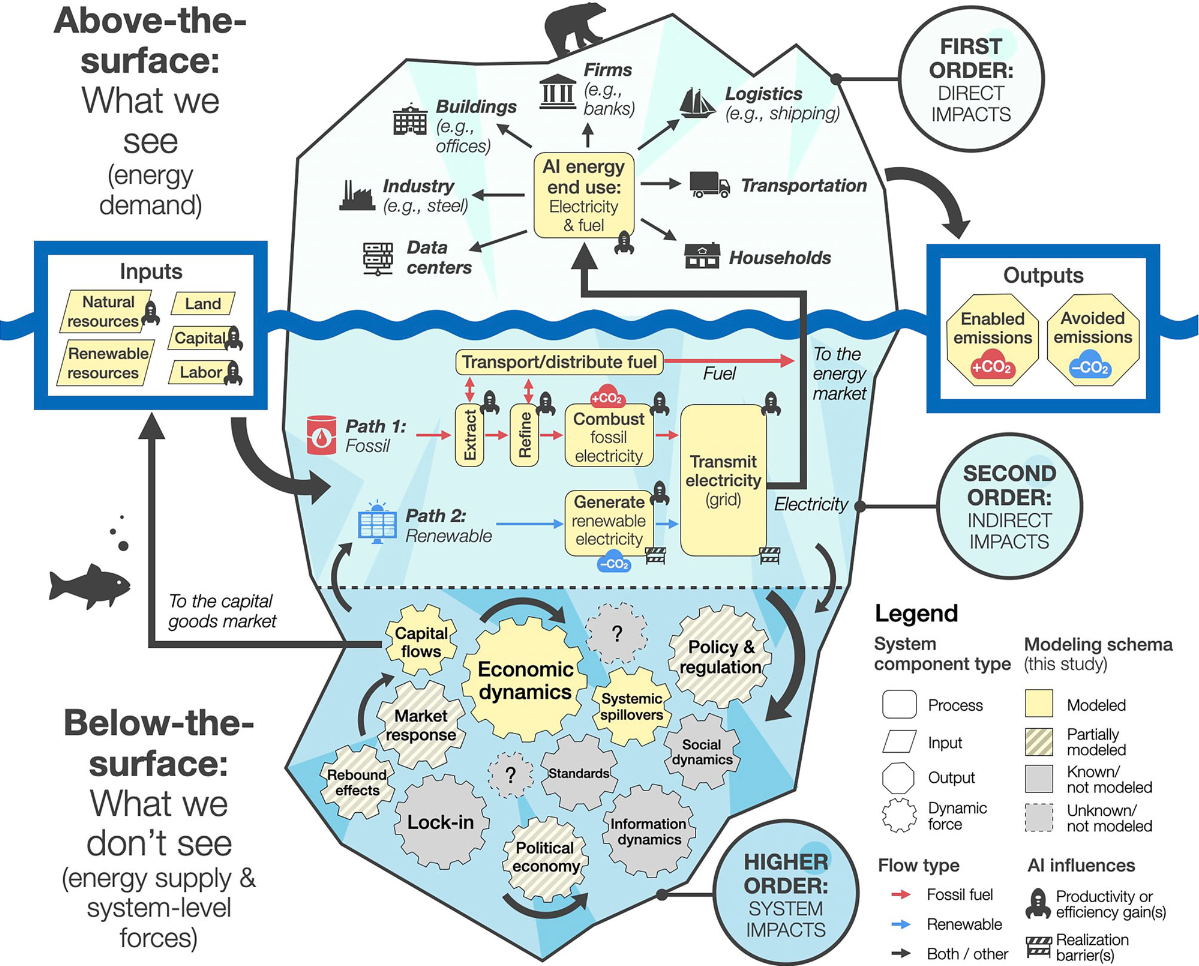
\includegraphics[width=.55\linewidth,keepaspectratio]{ai_energy_market_dynamics.png}
    \caption{AI energy-market dynamics \cite{Alpine2026}.}
\end{figure}

\end{frame}

\begin{frame}[fragile]{Der problematische Ressourcenverbrauch durch KI}

\begin{figure}
    \centering
    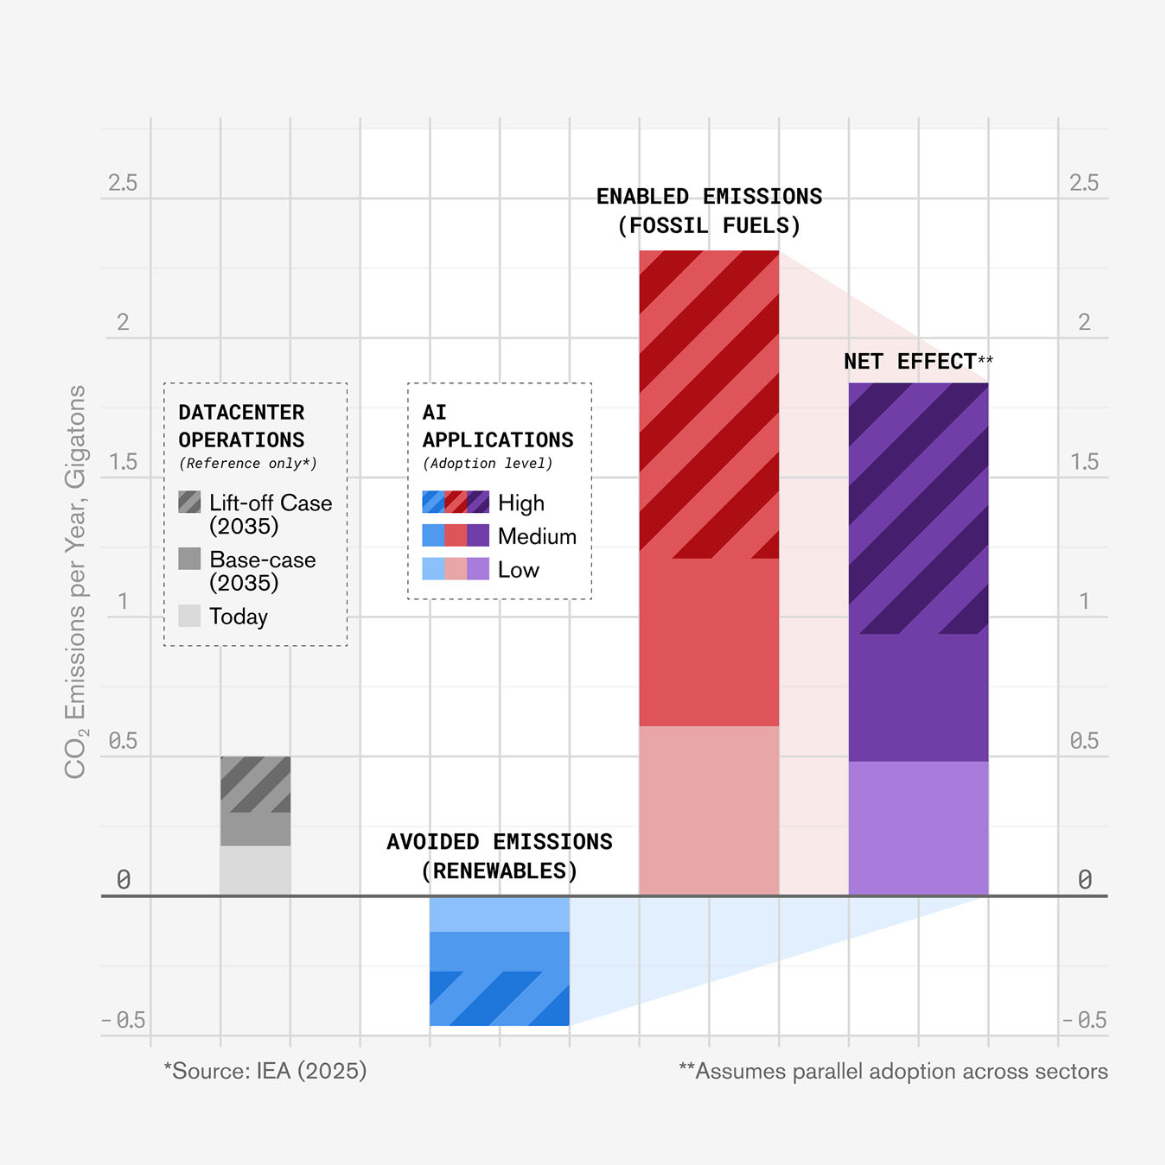
\includegraphics[width=.43\linewidth]{ai_mediated_productivity.png}
    \caption{Jährliche CO2-Emissionen durch KI heute und 2035 \cite{Alpine2026}.}
\end{figure}

% \slidesource{Rechenzentren: Zeitvergleich; KI-Anwendungen: statische Szenarien}
\end{frame}

\appendix
\begin{frame}[allowframebreaks]{Literatur}
\renewcommand*{\bibfont}{\scriptsize}
\printbibliography[heading=none]
\end{frame}
\end{document}
